\documentclass[twoside]{book}

% Packages required by doxygen
\usepackage{fixltx2e}
\usepackage{calc}
\usepackage{doxygen}
\usepackage[export]{adjustbox} % also loads graphicx
\usepackage{graphicx}
\usepackage[utf8]{inputenc}
\usepackage{makeidx}
\usepackage{multicol}
\usepackage{multirow}
\PassOptionsToPackage{warn}{textcomp}
\usepackage{textcomp}
\usepackage[nointegrals]{wasysym}
\usepackage[table]{xcolor}

% Font selection
\usepackage[T1]{fontenc}
\usepackage[scaled=.90]{helvet}
\usepackage{courier}
\usepackage{amssymb}
\usepackage{sectsty}
\renewcommand{\familydefault}{\sfdefault}
\allsectionsfont{%
  \fontseries{bc}\selectfont%
  \color{darkgray}%
}
\renewcommand{\DoxyLabelFont}{%
  \fontseries{bc}\selectfont%
  \color{darkgray}%
}
\newcommand{\+}{\discretionary{\mbox{\scriptsize$\hookleftarrow$}}{}{}}

% Page & text layout
\usepackage{geometry}
\geometry{%
  a4paper,%
  top=2.5cm,%
  bottom=2.5cm,%
  left=2.5cm,%
  right=2.5cm%
}
\tolerance=750
\hfuzz=15pt
\hbadness=750
\setlength{\emergencystretch}{15pt}
\setlength{\parindent}{0cm}
\setlength{\parskip}{3ex plus 2ex minus 2ex}
\makeatletter
\renewcommand{\paragraph}{%
  \@startsection{paragraph}{4}{0ex}{-1.0ex}{1.0ex}{%
    \normalfont\normalsize\bfseries\SS@parafont%
  }%
}
\renewcommand{\subparagraph}{%
  \@startsection{subparagraph}{5}{0ex}{-1.0ex}{1.0ex}{%
    \normalfont\normalsize\bfseries\SS@subparafont%
  }%
}
\makeatother

% Headers & footers
\usepackage{fancyhdr}
\pagestyle{fancyplain}
\fancyhead[LE]{\fancyplain{}{\bfseries\thepage}}
\fancyhead[CE]{\fancyplain{}{}}
\fancyhead[RE]{\fancyplain{}{\bfseries\leftmark}}
\fancyhead[LO]{\fancyplain{}{\bfseries\rightmark}}
\fancyhead[CO]{\fancyplain{}{}}
\fancyhead[RO]{\fancyplain{}{\bfseries\thepage}}
\fancyfoot[LE]{\fancyplain{}{}}
\fancyfoot[CE]{\fancyplain{}{}}
\fancyfoot[RE]{\fancyplain{}{\bfseries\scriptsize Generated by Doxygen }}
\fancyfoot[LO]{\fancyplain{}{\bfseries\scriptsize Generated by Doxygen }}
\fancyfoot[CO]{\fancyplain{}{}}
\fancyfoot[RO]{\fancyplain{}{}}
\renewcommand{\footrulewidth}{0.4pt}
\renewcommand{\chaptermark}[1]{%
  \markboth{#1}{}%
}
\renewcommand{\sectionmark}[1]{%
  \markright{\thesection\ #1}%
}

% Indices & bibliography
\usepackage{natbib}
\usepackage[titles]{tocloft}
\setcounter{tocdepth}{3}
\setcounter{secnumdepth}{5}
\makeindex

% Hyperlinks (required, but should be loaded last)
\usepackage{ifpdf}
\ifpdf
  \usepackage[pdftex,pagebackref=true]{hyperref}
\else
  \usepackage[ps2pdf,pagebackref=true]{hyperref}
\fi
\hypersetup{%
  colorlinks=true,%
  linkcolor=blue,%
  citecolor=blue,%
  unicode%
}

% Custom commands
\newcommand{\clearemptydoublepage}{%
  \newpage{\pagestyle{empty}\cleardoublepage}%
}

\usepackage{caption}
\captionsetup{labelsep=space,justification=centering,font={bf},singlelinecheck=off,skip=4pt,position=top}

%===== C O N T E N T S =====

\begin{document}

% Titlepage & ToC
\hypersetup{pageanchor=false,
             bookmarksnumbered=true,
             pdfencoding=unicode
            }
\pagenumbering{alph}
\begin{titlepage}
\vspace*{7cm}
\begin{center}%
{\Large Advanced Programming Exam -\/ Binary Search Tree }\\
\vspace*{1cm}
{\large Generated by Doxygen 1.8.13}\\
\end{center}
\end{titlepage}
\clearemptydoublepage
\pagenumbering{roman}
\tableofcontents
\clearemptydoublepage
\pagenumbering{arabic}
\hypersetup{pageanchor=true}

%--- Begin generated contents ---
\chapter{Hierarchical Index}
\section{Class Hierarchy}
This inheritance list is sorted roughly, but not completely, alphabetically\+:\begin{DoxyCompactList}
\item \contentsline{section}{Node\+Namespace\+:\+:B\+S\+T\+Node$<$ K, T $>$}{\pageref{class_node_namespace_1_1_b_s_t_node}}{}
\item \contentsline{section}{B\+S\+Tree$<$ K, T, C $>$}{\pageref{class_b_s_tree}}{}
\item \contentsline{section}{compareh}{\pageref{structcompareh}}{}
\item \contentsline{section}{error}{\pageref{structerror}}{}
\item \contentsline{section}{B\+S\+Tree$<$ K, T, C $>$\+:\+:Iterator}{\pageref{class_b_s_tree_1_1_iterator}}{}
\begin{DoxyCompactList}
\item \contentsline{section}{B\+S\+Tree$<$ K, T, C $>$\+:\+:Const\+Iterator}{\pageref{class_b_s_tree_1_1_const_iterator}}{}
\end{DoxyCompactList}
\item \contentsline{section}{Random\+Key}{\pageref{struct_random_key}}{}
\item \contentsline{section}{Random\+Key\+\_\+explicit}{\pageref{struct_random_key__explicit}}{}
\end{DoxyCompactList}

\chapter{Class Index}
\section{Class List}
Here are the classes, structs, unions and interfaces with brief descriptions\+:\begin{DoxyCompactList}
\item\contentsline{section}{\hyperlink{class_node_namespace_1_1_b_s_t_node}{Node\+Namespace\+::\+B\+S\+T\+Node$<$ K, T $>$} }{\pageref{class_node_namespace_1_1_b_s_t_node}}{}
\item\contentsline{section}{\hyperlink{class_b_s_tree}{B\+S\+Tree$<$ K, T, C $>$} }{\pageref{class_b_s_tree}}{}
\item\contentsline{section}{\hyperlink{structcompareh}{compareh} }{\pageref{structcompareh}}{}
\item\contentsline{section}{\hyperlink{class_b_s_tree_1_1_const_iterator}{B\+S\+Tree$<$ K, T, C $>$\+::\+Const\+Iterator} }{\pageref{class_b_s_tree_1_1_const_iterator}}{}
\item\contentsline{section}{\hyperlink{structerror}{error} }{\pageref{structerror}}{}
\item\contentsline{section}{\hyperlink{class_b_s_tree_1_1_iterator}{B\+S\+Tree$<$ K, T, C $>$\+::\+Iterator} }{\pageref{class_b_s_tree_1_1_iterator}}{}
\item\contentsline{section}{\hyperlink{struct_random_key}{Random\+Key} }{\pageref{struct_random_key}}{}
\item\contentsline{section}{\hyperlink{struct_random_key__explicit}{Random\+Key\+\_\+explicit} }{\pageref{struct_random_key__explicit}}{}
\end{DoxyCompactList}

\chapter{File Index}
\section{File List}
Here is a list of all documented files with brief descriptions\+:\begin{DoxyCompactList}
\item\contentsline{section}{/home/w-\/wilson/\+D\+S\+S\+C/first\+\_\+year/exam\+\_\+advanced/test/include/\hyperlink{_b_s_t_8h}{B\+S\+T.\+h} \\*B\+ST header file }{\pageref{_b_s_t_8h}}{}
\item\contentsline{section}{/home/w-\/wilson/\+D\+S\+S\+C/first\+\_\+year/exam\+\_\+advanced/test/src/{\bfseries B\+S\+T.\+hpp} }{\pageref{_b_s_t_8hpp}}{}
\item\contentsline{section}{/home/w-\/wilson/\+D\+S\+S\+C/first\+\_\+year/exam\+\_\+advanced/test/src/\hyperlink{main_8cc}{main.\+cc} \\*Main file for the exam }{\pageref{main_8cc}}{}
\end{DoxyCompactList}

\chapter{Class Documentation}
\hypertarget{class_node_namespace_1_1_b_s_t_node}{}\section{Node\+Namespace\+:\+:B\+S\+T\+Node$<$ K, T $>$ Class Template Reference}
\label{class_node_namespace_1_1_b_s_t_node}\index{Node\+Namespace\+::\+B\+S\+T\+Node$<$ K, T $>$@{Node\+Namespace\+::\+B\+S\+T\+Node$<$ K, T $>$}}


Collaboration diagram for Node\+Namespace\+:\+:B\+S\+T\+Node$<$ K, T $>$\+:\nopagebreak
\begin{figure}[H]
\begin{center}
\leavevmode
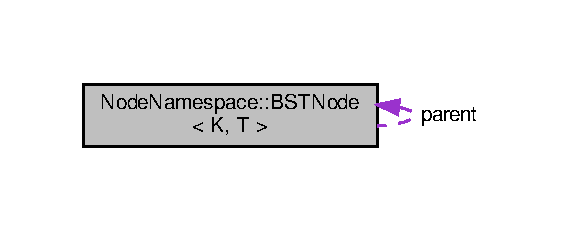
\includegraphics[width=270pt]{class_node_namespace_1_1_b_s_t_node__coll__graph}
\end{center}
\end{figure}
\subsection*{Public Member Functions}
\begin{DoxyCompactItemize}
\item 
\mbox{\Hypertarget{class_node_namespace_1_1_b_s_t_node_a783d05cdab47777a15e2b7b366db7d12}\label{class_node_namespace_1_1_b_s_t_node_a783d05cdab47777a15e2b7b366db7d12}} 
\hyperlink{class_node_namespace_1_1_b_s_t_node_a783d05cdab47777a15e2b7b366db7d12}{B\+S\+T\+Node} ()=default
\begin{DoxyCompactList}\small\item\em \hyperlink{class_node_namespace_1_1_b_s_t_node}{B\+S\+T\+Node} default constructor. \end{DoxyCompactList}\item 
\mbox{\Hypertarget{class_node_namespace_1_1_b_s_t_node_a867fb97b3ca84d805925b05f8daec0fa}\label{class_node_namespace_1_1_b_s_t_node_a867fb97b3ca84d805925b05f8daec0fa}} 
\hyperlink{class_node_namespace_1_1_b_s_t_node_a867fb97b3ca84d805925b05f8daec0fa}{B\+S\+T\+Node} (const std\+::pair$<$ const K, T $>$ \&data)
\begin{DoxyCompactList}\small\item\em \hyperlink{class_node_namespace_1_1_b_s_t_node}{B\+S\+T\+Node} constructor accepting a std\+::pair$<$\+K,\+T$>$ as input. \end{DoxyCompactList}\item 
\mbox{\Hypertarget{class_node_namespace_1_1_b_s_t_node_a77cc8b32b8edb62c20c5352ee897fee2}\label{class_node_namespace_1_1_b_s_t_node_a77cc8b32b8edb62c20c5352ee897fee2}} 
\hyperlink{class_node_namespace_1_1_b_s_t_node_a77cc8b32b8edb62c20c5352ee897fee2}{B\+S\+T\+Node} (const std\+::pair$<$ const K, T $>$ \&data, \hyperlink{class_node_namespace_1_1_b_s_t_node}{B\+S\+T\+Node} $\ast$\+\_\+parent)
\begin{DoxyCompactList}\small\item\em \hyperlink{class_node_namespace_1_1_b_s_t_node}{B\+S\+T\+Node} constructor accepting a std\+::pair$<$\+K,\+T$>$ and a pointer to the parent node as input. \end{DoxyCompactList}\item 
\mbox{\Hypertarget{class_node_namespace_1_1_b_s_t_node_ad039a31573c8f56b0c156b3799f8db52}\label{class_node_namespace_1_1_b_s_t_node_ad039a31573c8f56b0c156b3799f8db52}} 
\hyperlink{class_node_namespace_1_1_b_s_t_node_ad039a31573c8f56b0c156b3799f8db52}{$\sim$\+B\+S\+T\+Node} () noexcept=default
\begin{DoxyCompactList}\small\item\em Sefault \hyperlink{class_node_namespace_1_1_b_s_t_node}{B\+S\+T\+Node} destructor. \end{DoxyCompactList}\item 
bool \hyperlink{class_node_namespace_1_1_b_s_t_node_ae6572b47848a90ccf24fffd98e965888}{has\+L\+Child} () const noexcept
\begin{DoxyCompactList}\small\item\em Checks if the node has a left child. \end{DoxyCompactList}\item 
bool \hyperlink{class_node_namespace_1_1_b_s_t_node_a8850198713eafcc7033271ecb023b3bf}{has\+R\+Child} () const noexcept
\begin{DoxyCompactList}\small\item\em Checks if the node has a right child. \end{DoxyCompactList}\item 
\hyperlink{class_node_namespace_1_1_b_s_t_node}{B\+S\+T\+Node} $\ast$ \hyperlink{class_node_namespace_1_1_b_s_t_node_a706ff01acdd424c760594da6fa0cb645}{get\+\_\+next} () noexcept
\begin{DoxyCompactList}\small\item\em Returns a pointer to the next node, according to key order. \end{DoxyCompactList}\end{DoxyCompactItemize}
\subsection*{Public Attributes}
\begin{DoxyCompactItemize}
\item 
\mbox{\Hypertarget{class_node_namespace_1_1_b_s_t_node_a55b65280bcbe2668740e5240f6d11280}\label{class_node_namespace_1_1_b_s_t_node_a55b65280bcbe2668740e5240f6d11280}} 
std\+::pair$<$ const K, T $>$ {\bfseries content}
\item 
\mbox{\Hypertarget{class_node_namespace_1_1_b_s_t_node_ab69b41269379fb89daa298a98bb4ff22}\label{class_node_namespace_1_1_b_s_t_node_ab69b41269379fb89daa298a98bb4ff22}} 
std\+::unique\+\_\+ptr$<$ \hyperlink{class_node_namespace_1_1_b_s_t_node}{B\+S\+T\+Node} $>$ {\bfseries left}
\item 
\mbox{\Hypertarget{class_node_namespace_1_1_b_s_t_node_a8c6eb700b07ad11d6398ff3e89f3b743}\label{class_node_namespace_1_1_b_s_t_node_a8c6eb700b07ad11d6398ff3e89f3b743}} 
std\+::unique\+\_\+ptr$<$ \hyperlink{class_node_namespace_1_1_b_s_t_node}{B\+S\+T\+Node} $>$ {\bfseries right}
\item 
\mbox{\Hypertarget{class_node_namespace_1_1_b_s_t_node_ab7535b88780d30fda0c8a8664ba560f1}\label{class_node_namespace_1_1_b_s_t_node_ab7535b88780d30fda0c8a8664ba560f1}} 
\hyperlink{class_node_namespace_1_1_b_s_t_node}{B\+S\+T\+Node} $\ast$ {\bfseries parent}
\end{DoxyCompactItemize}


\subsection{Member Function Documentation}
\mbox{\Hypertarget{class_node_namespace_1_1_b_s_t_node_a706ff01acdd424c760594da6fa0cb645}\label{class_node_namespace_1_1_b_s_t_node_a706ff01acdd424c760594da6fa0cb645}} 
\index{Node\+Namespace\+::\+B\+S\+T\+Node@{Node\+Namespace\+::\+B\+S\+T\+Node}!get\+\_\+next@{get\+\_\+next}}
\index{get\+\_\+next@{get\+\_\+next}!Node\+Namespace\+::\+B\+S\+T\+Node@{Node\+Namespace\+::\+B\+S\+T\+Node}}
\subsubsection{\texorpdfstring{get\+\_\+next()}{get\_next()}}
{\footnotesize\ttfamily template$<$typename K , typename T $>$ \\
\hyperlink{class_node_namespace_1_1_b_s_t_node}{Node\+Namespace\+::\+B\+S\+T\+Node}$<$ K, T $>$ $\ast$ \hyperlink{class_node_namespace_1_1_b_s_t_node}{Node\+Namespace\+::\+B\+S\+T\+Node}$<$ K, T $>$\+::get\+\_\+next (\begin{DoxyParamCaption}{ }\end{DoxyParamCaption})\hspace{0.3cm}{\ttfamily [noexcept]}}



Returns a pointer to the next node, according to key order. 


\begin{DoxyParams}{Parameters}
{\em none} & \\
\hline
\end{DoxyParams}
\begin{DoxyReturn}{Returns}
Pointer to the next node. 
\end{DoxyReturn}
\mbox{\Hypertarget{class_node_namespace_1_1_b_s_t_node_ae6572b47848a90ccf24fffd98e965888}\label{class_node_namespace_1_1_b_s_t_node_ae6572b47848a90ccf24fffd98e965888}} 
\index{Node\+Namespace\+::\+B\+S\+T\+Node@{Node\+Namespace\+::\+B\+S\+T\+Node}!has\+L\+Child@{has\+L\+Child}}
\index{has\+L\+Child@{has\+L\+Child}!Node\+Namespace\+::\+B\+S\+T\+Node@{Node\+Namespace\+::\+B\+S\+T\+Node}}
\subsubsection{\texorpdfstring{has\+L\+Child()}{hasLChild()}}
{\footnotesize\ttfamily template$<$typename K, typename T$>$ \\
bool \hyperlink{class_node_namespace_1_1_b_s_t_node}{Node\+Namespace\+::\+B\+S\+T\+Node}$<$ K, T $>$\+::has\+L\+Child (\begin{DoxyParamCaption}{ }\end{DoxyParamCaption}) const\hspace{0.3cm}{\ttfamily [inline]}, {\ttfamily [noexcept]}}



Checks if the node has a left child. 


\begin{DoxyParams}{Parameters}
{\em none} & \\
\hline
\end{DoxyParams}
\begin{DoxyReturn}{Returns}
True if the node has a left child, False otherwise. 
\end{DoxyReturn}
\mbox{\Hypertarget{class_node_namespace_1_1_b_s_t_node_a8850198713eafcc7033271ecb023b3bf}\label{class_node_namespace_1_1_b_s_t_node_a8850198713eafcc7033271ecb023b3bf}} 
\index{Node\+Namespace\+::\+B\+S\+T\+Node@{Node\+Namespace\+::\+B\+S\+T\+Node}!has\+R\+Child@{has\+R\+Child}}
\index{has\+R\+Child@{has\+R\+Child}!Node\+Namespace\+::\+B\+S\+T\+Node@{Node\+Namespace\+::\+B\+S\+T\+Node}}
\subsubsection{\texorpdfstring{has\+R\+Child()}{hasRChild()}}
{\footnotesize\ttfamily template$<$typename K, typename T$>$ \\
bool \hyperlink{class_node_namespace_1_1_b_s_t_node}{Node\+Namespace\+::\+B\+S\+T\+Node}$<$ K, T $>$\+::has\+R\+Child (\begin{DoxyParamCaption}{ }\end{DoxyParamCaption}) const\hspace{0.3cm}{\ttfamily [inline]}, {\ttfamily [noexcept]}}



Checks if the node has a right child. 


\begin{DoxyParams}{Parameters}
{\em none} & \\
\hline
\end{DoxyParams}
\begin{DoxyReturn}{Returns}
True if the node has a right child, False otherwise. 
\end{DoxyReturn}


The documentation for this class was generated from the following files\+:\begin{DoxyCompactItemize}
\item 
/home/w-\/wilson/\+D\+S\+S\+C/first\+\_\+year/exam\+\_\+advanced/test/include/\hyperlink{_b_s_t_8h}{B\+S\+T.\+h}\item 
/home/w-\/wilson/\+D\+S\+S\+C/first\+\_\+year/exam\+\_\+advanced/test/src/B\+S\+T.\+hpp\end{DoxyCompactItemize}

\hypertarget{class_b_s_tree}{}\section{B\+S\+Tree$<$ K, T, C $>$ Class Template Reference}
\label{class_b_s_tree}\index{B\+S\+Tree$<$ K, T, C $>$@{B\+S\+Tree$<$ K, T, C $>$}}


{\ttfamily \#include $<$B\+S\+T.\+h$>$}

\subsection*{Classes}
\begin{DoxyCompactItemize}
\item 
class \hyperlink{class_b_s_tree_1_1_const_iterator}{Const\+Iterator}
\item 
class \hyperlink{class_b_s_tree_1_1_iterator}{Iterator}
\end{DoxyCompactItemize}
\subsection*{Public Member Functions}
\begin{DoxyCompactItemize}
\item 
const int \& \hyperlink{class_b_s_tree_a176f1ccfb16c72f653d27c0a8a02fbb5}{size\+\_\+of} () const noexcept
\begin{DoxyCompactList}\small\item\em Returns the number of elements of the tree. \end{DoxyCompactList}\item 
bool \hyperlink{class_b_s_tree_a8002c1bc948d8ef1085fb53949562fc0}{is\+\_\+empty} () const noexcept
\begin{DoxyCompactList}\small\item\em Check if the tree is empty. \end{DoxyCompactList}\item 
const \hyperlink{class_node_namespace_1_1_b_s_t_node}{B\+S\+T\+Node}$<$ K, T $>$ $\ast$ \hyperlink{class_b_s_tree_add1b6b6c2b9b5a871d6ae06ba2ab174f}{get\+\_\+root} () const
\begin{DoxyCompactList}\small\item\em Returns a pointer to the root node. \end{DoxyCompactList}\item 
\mbox{\Hypertarget{class_b_s_tree_a31f5f4929f634ab6eeeed262158a407f}\label{class_b_s_tree_a31f5f4929f634ab6eeeed262158a407f}} 
\hyperlink{class_b_s_tree_a31f5f4929f634ab6eeeed262158a407f}{B\+S\+Tree} ()=default
\begin{DoxyCompactList}\small\item\em Default \hyperlink{class_b_s_tree}{B\+S\+Tree} constructor. \end{DoxyCompactList}\item 
\mbox{\Hypertarget{class_b_s_tree_a4c7cc79e77368b2196be5463ce51dabb}\label{class_b_s_tree_a4c7cc79e77368b2196be5463ce51dabb}} 
\hyperlink{class_b_s_tree_a4c7cc79e77368b2196be5463ce51dabb}{B\+S\+Tree} (const K \&key, const T \&value, C comp=C\{\})
\begin{DoxyCompactList}\small\item\em \hyperlink{class_b_s_tree}{B\+S\+Tree} constructor accepting a key and a value, inserted as root. \end{DoxyCompactList}\item 
\mbox{\Hypertarget{class_b_s_tree_aa688700e2b3298d2c59ecb505522daf2}\label{class_b_s_tree_aa688700e2b3298d2c59ecb505522daf2}} 
\hyperlink{class_b_s_tree_aa688700e2b3298d2c59ecb505522daf2}{B\+S\+Tree} (const std\+::pair$<$ const K, T $>$ \&data, C comp=C\{\})
\begin{DoxyCompactList}\small\item\em \hyperlink{class_b_s_tree}{B\+S\+Tree} constructor accepting a std\+::pair$<$key,value$>$ inserted as root. \end{DoxyCompactList}\item 
\mbox{\Hypertarget{class_b_s_tree_a875eb7debc36c3972bc9fb6b486cd64d}\label{class_b_s_tree_a875eb7debc36c3972bc9fb6b486cd64d}} 
\hyperlink{class_b_s_tree_a875eb7debc36c3972bc9fb6b486cd64d}{$\sim$\+B\+S\+Tree} () noexcept=default
\begin{DoxyCompactList}\small\item\em Default \hyperlink{class_b_s_tree}{B\+S\+Tree} destructor. \end{DoxyCompactList}\item 
\hyperlink{class_b_s_tree_ab02cf77eca992f95d44c4ada43a914c0}{B\+S\+Tree} (const \hyperlink{class_b_s_tree}{B\+S\+Tree} \&t)
\begin{DoxyCompactList}\small\item\em Copy constructor for a \hyperlink{class_b_s_tree}{B\+S\+Tree}. Calls the auxiliary function \hyperlink{class_b_s_tree_ad34bd4cfe46ab5a5376cc242b1901f2b}{copy\+\_\+tree()} which performs a deep copy of the tree. \end{DoxyCompactList}\item 
\hyperlink{class_b_s_tree}{B\+S\+Tree} \& \hyperlink{class_b_s_tree_a51e883c53f2604130eeabecc73a2a95a}{operator=} (const \hyperlink{class_b_s_tree}{B\+S\+Tree} \&t)
\begin{DoxyCompactList}\small\item\em Copy assignment of a \hyperlink{class_b_s_tree}{B\+S\+Tree}. \end{DoxyCompactList}\item 
\mbox{\Hypertarget{class_b_s_tree_a6f8861897a87ab1944edbaf7754648b4}\label{class_b_s_tree_a6f8861897a87ab1944edbaf7754648b4}} 
\hyperlink{class_b_s_tree_a6f8861897a87ab1944edbaf7754648b4}{B\+S\+Tree} (\hyperlink{class_b_s_tree}{B\+S\+Tree}$<$ K, T, C $>$ \&\&) noexcept=default
\begin{DoxyCompactList}\small\item\em Default move constructor for a \hyperlink{class_b_s_tree}{B\+S\+Tree}. \end{DoxyCompactList}\item 
\mbox{\Hypertarget{class_b_s_tree_a555de0952655377d903ecbc1ce6bdec3}\label{class_b_s_tree_a555de0952655377d903ecbc1ce6bdec3}} 
\hyperlink{class_b_s_tree}{B\+S\+Tree}$<$ K, T, C $>$ \& \hyperlink{class_b_s_tree_a555de0952655377d903ecbc1ce6bdec3}{operator=} (\hyperlink{class_b_s_tree}{B\+S\+Tree}$<$ K, T, C $>$ \&\&) noexcept=default
\begin{DoxyCompactList}\small\item\em Default move assignment for a \hyperlink{class_b_s_tree}{B\+S\+Tree}. \end{DoxyCompactList}\item 
\hyperlink{class_b_s_tree_1_1_iterator}{Iterator} \hyperlink{class_b_s_tree_afb41cae2749cded61f805bb1b902f811}{begin} ()
\begin{DoxyCompactList}\small\item\em first element for iterating a \hyperlink{class_b_s_tree}{B\+S\+Tree}. \end{DoxyCompactList}\item 
\hyperlink{class_b_s_tree_1_1_iterator}{Iterator} \hyperlink{class_b_s_tree_af08ce4b341b8503949ede9d4e6af8c8b}{end} ()
\begin{DoxyCompactList}\small\item\em last element for iterating a \hyperlink{class_b_s_tree}{B\+S\+Tree} \end{DoxyCompactList}\item 
\hyperlink{class_b_s_tree_1_1_const_iterator}{Const\+Iterator} \hyperlink{class_b_s_tree_a575273bc2b272f20f8b6802f2b0a756f}{cbegin} () const
\begin{DoxyCompactList}\small\item\em first element for iterating a \hyperlink{class_b_s_tree}{B\+S\+Tree}. \end{DoxyCompactList}\item 
\hyperlink{class_b_s_tree_1_1_const_iterator}{Const\+Iterator} \hyperlink{class_b_s_tree_a562638580a40643c76913e51dd06c13b}{cend} () const
\begin{DoxyCompactList}\small\item\em last element for iterating a \hyperlink{class_b_s_tree}{B\+S\+Tree} \end{DoxyCompactList}\item 
bool \hyperlink{class_b_s_tree_a23746c31f7583acad81c9b7f08159003}{insert} (const std\+::pair$<$ const K, T $>$ \&data)
\begin{DoxyCompactList}\small\item\em Inserts a B\+S\+T\+Node passing a std\+::pair$<$key,value$>$. Calls position\+\_\+of(key) to find where the node should be appended. If the key is already present, does nothing. Otherwise a new node is created. \end{DoxyCompactList}\item 
bool \hyperlink{class_b_s_tree_a00ca543914dbdaa89b9c9f6fae7d6555}{insert} (const K \&key, const T \&value)
\begin{DoxyCompactList}\small\item\em Inserts a node passing a key and a value separately. \end{DoxyCompactList}\item 
\hyperlink{class_b_s_tree_1_1_iterator}{Iterator} \hyperlink{class_b_s_tree_a739cf62b2b972cd063928357dd2aba9a}{find} (const K \&key) const
\begin{DoxyCompactList}\small\item\em Returns, if found, an iterator to the node labelled by key. \end{DoxyCompactList}\item 
void \hyperlink{class_b_s_tree_ae5362c45ed2bc96c9c72fdef689bd078}{clear} () noexcept
\begin{DoxyCompactList}\small\item\em Wipes out the tree. Resets the root to nullptr, causing all the other nodes to be deleted. The tree is left uninitialized, but still usable. \end{DoxyCompactList}\item 
void \hyperlink{class_b_s_tree_a468dcc29b6786ddc5de05c314d644ce1}{print} () const
\begin{DoxyCompactList}\small\item\em Prints the value in all the nodes, traversing the tree in order. \end{DoxyCompactList}\item 
void \hyperlink{class_b_s_tree_a955848e883b93312a467c0ee103db8df}{balance} ()
\begin{DoxyCompactList}\small\item\em Balances the tree. \end{DoxyCompactList}\item 
T \& \hyperlink{class_b_s_tree_adb6e522a0dbbedd33ad21724b4dca0f6}{operator\mbox{[}$\,$\mbox{]}} (const K \&k)
\begin{DoxyCompactList}\small\item\em Operator \mbox{[}\mbox{]} to access/insert a B\+S\+T\+Node. Returns the value associated with key if found. Otherwise, appends a node with the desired key and the default value. \end{DoxyCompactList}\item 
\mbox{\Hypertarget{class_b_s_tree_a265ffc422b631fee4e51531db590a957}\label{class_b_s_tree_a265ffc422b631fee4e51531db590a957}} 
const T \& {\bfseries operator\mbox{[}$\,$\mbox{]}} (const K \&k) const
\item 
const T \& \hyperlink{class_b_s_tree_a8b5a7600d91dee310ece37c10cbceb6a}{square\+\_\+bracket\+\_\+test} (const K \&key) const
\begin{DoxyCompactList}\small\item\em Operator $<$$<$ to print a \hyperlink{class_b_s_tree}{B\+S\+Tree}. \end{DoxyCompactList}\end{DoxyCompactItemize}
\subsection*{Public Attributes}
\begin{DoxyCompactItemize}
\item 
\mbox{\Hypertarget{class_b_s_tree_abf0711d0f2e62ed4a6fee153ad717833}\label{class_b_s_tree_abf0711d0f2e62ed4a6fee153ad717833}} 
C {\bfseries compare\+\_\+f}
\end{DoxyCompactItemize}
\subsection*{Private Member Functions}
\begin{DoxyCompactItemize}
\item 
\hyperlink{class_node_namespace_1_1_b_s_t_node}{B\+S\+T\+Node}$<$ K, T $>$ $\ast$ \hyperlink{class_b_s_tree_ab77c72f33d88ca3311286744370138bb}{get\+\_\+most\+\_\+left} (\hyperlink{class_node_namespace_1_1_b_s_t_node}{B\+S\+T\+Node}$<$ K, T $>$ $\ast$curr\+Node) const noexcept
\begin{DoxyCompactList}\small\item\em Returns a pointer to the leftmost element of a subtree. \end{DoxyCompactList}\item 
void \hyperlink{class_b_s_tree_ad34bd4cfe46ab5a5376cc242b1901f2b}{copy\+\_\+tree} (const \hyperlink{class_node_namespace_1_1_b_s_t_node}{B\+S\+T\+Node}$<$ K, T $>$ $\ast$curr\+Node)
\begin{DoxyCompactList}\small\item\em Auxiliary function for the copy constructor, performs a deep copy. \end{DoxyCompactList}\item 
\hyperlink{class_b_s_tree_1_1_iterator}{Iterator} \hyperlink{class_b_s_tree_a0a386f0ffde9a0fe2e5df8562b719184}{position\+\_\+of} (const K \&key) const
\begin{DoxyCompactList}\small\item\em Auxiliary function for the insert(key, value) and find(key) methods. \end{DoxyCompactList}\item 
void \hyperlink{class_b_s_tree_a3ae6d9b52f23edb005289f52200b0b70}{balance} (std\+::vector$<$ std\+::pair$<$ const K, T $>$$>$ \&vine, const int \&\hyperlink{class_b_s_tree_afb41cae2749cded61f805bb1b902f811}{begin}, const int \&\hyperlink{class_b_s_tree_af08ce4b341b8503949ede9d4e6af8c8b}{end})
\begin{DoxyCompactList}\small\item\em Iteratively builds a balanced tree starting from an ordered std\+::vector. \end{DoxyCompactList}\end{DoxyCompactItemize}
\subsection*{Private Attributes}
\begin{DoxyCompactItemize}
\item 
\mbox{\Hypertarget{class_b_s_tree_aa0d1b3c092ac0616ed758c37eeae28ae}\label{class_b_s_tree_aa0d1b3c092ac0616ed758c37eeae28ae}} 
std\+::unique\+\_\+ptr$<$ \hyperlink{class_node_namespace_1_1_b_s_t_node}{B\+S\+T\+Node}$<$ K, T $>$ $>$ {\bfseries root} = nullptr
\item 
\mbox{\Hypertarget{class_b_s_tree_a32a650287c9c6ac09282d0c12a34997b}\label{class_b_s_tree_a32a650287c9c6ac09282d0c12a34997b}} 
int {\bfseries size} = 0
\end{DoxyCompactItemize}


\subsection{Detailed Description}
\subsubsection*{template$<$typename K, typename T, typename C = std\+::less$<$\+K$>$$>$\newline
class B\+S\+Tree$<$ K, T, C $>$}

Binary Search Tree implementation.

Implementation of a Binary Search Tree. The tree is made of nodes which store a key/value pair. It requires a compare structure to order keys. If none is provided, it uses std\+::less$<$\+K$>$, where K is the key type. 

\subsection{Constructor \& Destructor Documentation}
\mbox{\Hypertarget{class_b_s_tree_ab02cf77eca992f95d44c4ada43a914c0}\label{class_b_s_tree_ab02cf77eca992f95d44c4ada43a914c0}} 
\index{B\+S\+Tree@{B\+S\+Tree}!B\+S\+Tree@{B\+S\+Tree}}
\index{B\+S\+Tree@{B\+S\+Tree}!B\+S\+Tree@{B\+S\+Tree}}
\subsubsection{\texorpdfstring{B\+S\+Tree()}{BSTree()}}
{\footnotesize\ttfamily template$<$typename K, typename T, typename C = std\+::less$<$\+K$>$$>$ \\
\hyperlink{class_b_s_tree}{B\+S\+Tree}$<$ K, T, C $>$\+::\hyperlink{class_b_s_tree}{B\+S\+Tree} (\begin{DoxyParamCaption}\item[{const \hyperlink{class_b_s_tree}{B\+S\+Tree}$<$ K, T, C $>$ \&}]{t }\end{DoxyParamCaption})\hspace{0.3cm}{\ttfamily [inline]}}



Copy constructor for a \hyperlink{class_b_s_tree}{B\+S\+Tree}. Calls the auxiliary function \hyperlink{class_b_s_tree_ad34bd4cfe46ab5a5376cc242b1901f2b}{copy\+\_\+tree()} which performs a deep copy of the tree. 


\begin{DoxyParams}{Parameters}
{\em t} & \hyperlink{class_b_s_tree}{B\+S\+Tree} to be copied, passed by const reference. \\
\hline
\end{DoxyParams}


\subsection{Member Function Documentation}
\mbox{\Hypertarget{class_b_s_tree_a955848e883b93312a467c0ee103db8df}\label{class_b_s_tree_a955848e883b93312a467c0ee103db8df}} 
\index{B\+S\+Tree@{B\+S\+Tree}!balance@{balance}}
\index{balance@{balance}!B\+S\+Tree@{B\+S\+Tree}}
\subsubsection{\texorpdfstring{balance()}{balance()}\hspace{0.1cm}{\footnotesize\ttfamily [1/2]}}
{\footnotesize\ttfamily template$<$typename K , typename T , typename C $>$ \\
void \hyperlink{class_b_s_tree}{B\+S\+Tree}$<$ K, T, C $>$\+::balance (\begin{DoxyParamCaption}{ }\end{DoxyParamCaption})}



Balances the tree. 

The tree is linearized into a vector of std\+::pair$<$key,value$>$. Then calls \hyperlink{class_b_s_tree_ae5362c45ed2bc96c9c72fdef689bd078}{clear()} and the auxiliary function balance(vector, begin, end).


\begin{DoxyParams}{Parameters}
{\em none} & \\
\hline
\end{DoxyParams}
\begin{DoxyReturn}{Returns}
none 
\end{DoxyReturn}
\mbox{\Hypertarget{class_b_s_tree_a3ae6d9b52f23edb005289f52200b0b70}\label{class_b_s_tree_a3ae6d9b52f23edb005289f52200b0b70}} 
\index{B\+S\+Tree@{B\+S\+Tree}!balance@{balance}}
\index{balance@{balance}!B\+S\+Tree@{B\+S\+Tree}}
\subsubsection{\texorpdfstring{balance()}{balance()}\hspace{0.1cm}{\footnotesize\ttfamily [2/2]}}
{\footnotesize\ttfamily template$<$typename K , typename T , typename C $>$ \\
void \hyperlink{class_b_s_tree}{B\+S\+Tree}$<$ K, T, C $>$\+::balance (\begin{DoxyParamCaption}\item[{std\+::vector$<$ std\+::pair$<$ const K, T $>$$>$ \&}]{vine,  }\item[{const int \&}]{begin,  }\item[{const int \&}]{end }\end{DoxyParamCaption})\hspace{0.3cm}{\ttfamily [private]}}



Iteratively builds a balanced tree starting from an ordered std\+::vector. 

Builds a balanced tree appending the middle element of the vector, and then iteratively calling itself to append the middle element of the two halves, with begin and end as the extremes of the halves.


\begin{DoxyParams}{Parameters}
{\em vine} & std\+::vector of std\+::pair$<$key, value$>$ ordered by key. \\
\hline
{\em begin} & index of the first element to be considered. \\
\hline
{\em end} & index of the last element to be considered. \\
\hline
\end{DoxyParams}
\mbox{\Hypertarget{class_b_s_tree_afb41cae2749cded61f805bb1b902f811}\label{class_b_s_tree_afb41cae2749cded61f805bb1b902f811}} 
\index{B\+S\+Tree@{B\+S\+Tree}!begin@{begin}}
\index{begin@{begin}!B\+S\+Tree@{B\+S\+Tree}}
\subsubsection{\texorpdfstring{begin()}{begin()}}
{\footnotesize\ttfamily template$<$typename K, typename T, typename C = std\+::less$<$\+K$>$$>$ \\
\hyperlink{class_b_s_tree_1_1_iterator}{Iterator} \hyperlink{class_b_s_tree}{B\+S\+Tree}$<$ K, T, C $>$\+::begin (\begin{DoxyParamCaption}{ }\end{DoxyParamCaption})\hspace{0.3cm}{\ttfamily [inline]}}



first element for iterating a \hyperlink{class_b_s_tree}{B\+S\+Tree}. 

\begin{DoxyReturn}{Returns}
iterator to the leftmost node. 
\end{DoxyReturn}
\mbox{\Hypertarget{class_b_s_tree_a575273bc2b272f20f8b6802f2b0a756f}\label{class_b_s_tree_a575273bc2b272f20f8b6802f2b0a756f}} 
\index{B\+S\+Tree@{B\+S\+Tree}!cbegin@{cbegin}}
\index{cbegin@{cbegin}!B\+S\+Tree@{B\+S\+Tree}}
\subsubsection{\texorpdfstring{cbegin()}{cbegin()}}
{\footnotesize\ttfamily template$<$typename K, typename T, typename C = std\+::less$<$\+K$>$$>$ \\
\hyperlink{class_b_s_tree_1_1_const_iterator}{Const\+Iterator} \hyperlink{class_b_s_tree}{B\+S\+Tree}$<$ K, T, C $>$\+::cbegin (\begin{DoxyParamCaption}{ }\end{DoxyParamCaption}) const\hspace{0.3cm}{\ttfamily [inline]}}



first element for iterating a \hyperlink{class_b_s_tree}{B\+S\+Tree}. 

\begin{DoxyReturn}{Returns}
constiterator to the leftmost node. 
\end{DoxyReturn}
\mbox{\Hypertarget{class_b_s_tree_a562638580a40643c76913e51dd06c13b}\label{class_b_s_tree_a562638580a40643c76913e51dd06c13b}} 
\index{B\+S\+Tree@{B\+S\+Tree}!cend@{cend}}
\index{cend@{cend}!B\+S\+Tree@{B\+S\+Tree}}
\subsubsection{\texorpdfstring{cend()}{cend()}}
{\footnotesize\ttfamily template$<$typename K, typename T, typename C = std\+::less$<$\+K$>$$>$ \\
\hyperlink{class_b_s_tree_1_1_const_iterator}{Const\+Iterator} \hyperlink{class_b_s_tree}{B\+S\+Tree}$<$ K, T, C $>$\+::cend (\begin{DoxyParamCaption}{ }\end{DoxyParamCaption}) const\hspace{0.3cm}{\ttfamily [inline]}}



last element for iterating a \hyperlink{class_b_s_tree}{B\+S\+Tree} 

\begin{DoxyReturn}{Returns}
cosntiterator to nullptr. 
\end{DoxyReturn}
\mbox{\Hypertarget{class_b_s_tree_ae5362c45ed2bc96c9c72fdef689bd078}\label{class_b_s_tree_ae5362c45ed2bc96c9c72fdef689bd078}} 
\index{B\+S\+Tree@{B\+S\+Tree}!clear@{clear}}
\index{clear@{clear}!B\+S\+Tree@{B\+S\+Tree}}
\subsubsection{\texorpdfstring{clear()}{clear()}}
{\footnotesize\ttfamily template$<$typename K , typename T , typename C $>$ \\
void \hyperlink{class_b_s_tree}{B\+S\+Tree}$<$ K, T, C $>$\+::clear (\begin{DoxyParamCaption}{ }\end{DoxyParamCaption})\hspace{0.3cm}{\ttfamily [noexcept]}}



Wipes out the tree. Resets the root to nullptr, causing all the other nodes to be deleted. The tree is left uninitialized, but still usable. 


\begin{DoxyParams}{Parameters}
{\em none} & \\
\hline
\end{DoxyParams}
\begin{DoxyReturn}{Returns}
none 
\end{DoxyReturn}
\mbox{\Hypertarget{class_b_s_tree_ad34bd4cfe46ab5a5376cc242b1901f2b}\label{class_b_s_tree_ad34bd4cfe46ab5a5376cc242b1901f2b}} 
\index{B\+S\+Tree@{B\+S\+Tree}!copy\+\_\+tree@{copy\+\_\+tree}}
\index{copy\+\_\+tree@{copy\+\_\+tree}!B\+S\+Tree@{B\+S\+Tree}}
\subsubsection{\texorpdfstring{copy\+\_\+tree()}{copy\_tree()}}
{\footnotesize\ttfamily template$<$typename K , typename T , typename C $>$ \\
void \hyperlink{class_b_s_tree}{B\+S\+Tree}$<$ K, T, C $>$\+::copy\+\_\+tree (\begin{DoxyParamCaption}\item[{const \hyperlink{class_node_namespace_1_1_b_s_t_node}{B\+S\+T\+Node}$<$ K, T $>$ $\ast$}]{curr\+Node }\end{DoxyParamCaption})\hspace{0.3cm}{\ttfamily [private]}}



Auxiliary function for the copy constructor, performs a deep copy. 


\begin{DoxyParams}{Parameters}
{\em curr\+Node} & Pointer to the root of the subtree to be copied. \\
\hline
\end{DoxyParams}
\begin{DoxyReturn}{Returns}
none 
\end{DoxyReturn}
\mbox{\Hypertarget{class_b_s_tree_af08ce4b341b8503949ede9d4e6af8c8b}\label{class_b_s_tree_af08ce4b341b8503949ede9d4e6af8c8b}} 
\index{B\+S\+Tree@{B\+S\+Tree}!end@{end}}
\index{end@{end}!B\+S\+Tree@{B\+S\+Tree}}
\subsubsection{\texorpdfstring{end()}{end()}}
{\footnotesize\ttfamily template$<$typename K, typename T, typename C = std\+::less$<$\+K$>$$>$ \\
\hyperlink{class_b_s_tree_1_1_iterator}{Iterator} \hyperlink{class_b_s_tree}{B\+S\+Tree}$<$ K, T, C $>$\+::end (\begin{DoxyParamCaption}{ }\end{DoxyParamCaption})\hspace{0.3cm}{\ttfamily [inline]}}



last element for iterating a \hyperlink{class_b_s_tree}{B\+S\+Tree} 

\begin{DoxyReturn}{Returns}
iterator to nullptr. 
\end{DoxyReturn}
\mbox{\Hypertarget{class_b_s_tree_a739cf62b2b972cd063928357dd2aba9a}\label{class_b_s_tree_a739cf62b2b972cd063928357dd2aba9a}} 
\index{B\+S\+Tree@{B\+S\+Tree}!find@{find}}
\index{find@{find}!B\+S\+Tree@{B\+S\+Tree}}
\subsubsection{\texorpdfstring{find()}{find()}}
{\footnotesize\ttfamily template$<$typename K , typename T , typename C $>$ \\
\hyperlink{class_b_s_tree}{B\+S\+Tree}$<$ K, T, C $>$\+::\hyperlink{class_b_s_tree_1_1_iterator}{Iterator} \hyperlink{class_b_s_tree}{B\+S\+Tree}$<$ K, T, C $>$\+::find (\begin{DoxyParamCaption}\item[{const K \&}]{key }\end{DoxyParamCaption}) const}



Returns, if found, an iterator to the node labelled by key. 

Calls the auxiliary function position\+\_\+of(key) which returns, if key is found, an iterator pointing to the node that contains key. If the key is not found or the \hyperlink{class_b_s_tree}{B\+S\+Tree} is empty, retuns a \hyperlink{class_b_s_tree_1_1_const_iterator}{Const\+Iterator} to nullptr.


\begin{DoxyParams}{Parameters}
{\em key} & Key to be found. \\
\hline
\end{DoxyParams}
\begin{DoxyReturn}{Returns}
\hyperlink{class_b_s_tree_1_1_iterator}{Iterator} to the node containing the requested key or to nullptr. 
\end{DoxyReturn}
\mbox{\Hypertarget{class_b_s_tree_ab77c72f33d88ca3311286744370138bb}\label{class_b_s_tree_ab77c72f33d88ca3311286744370138bb}} 
\index{B\+S\+Tree@{B\+S\+Tree}!get\+\_\+most\+\_\+left@{get\+\_\+most\+\_\+left}}
\index{get\+\_\+most\+\_\+left@{get\+\_\+most\+\_\+left}!B\+S\+Tree@{B\+S\+Tree}}
\subsubsection{\texorpdfstring{get\+\_\+most\+\_\+left()}{get\_most\_left()}}
{\footnotesize\ttfamily template$<$typename K , typename T , typename C $>$ \\
\hyperlink{class_node_namespace_1_1_b_s_t_node}{B\+S\+T\+Node}$<$ K, T $>$ $\ast$ \hyperlink{class_b_s_tree}{B\+S\+Tree}$<$ K, T, C $>$\+::get\+\_\+most\+\_\+left (\begin{DoxyParamCaption}\item[{\hyperlink{class_node_namespace_1_1_b_s_t_node}{B\+S\+T\+Node}$<$ K, T $>$ $\ast$}]{curr\+Node }\end{DoxyParamCaption}) const\hspace{0.3cm}{\ttfamily [private]}, {\ttfamily [noexcept]}}



Returns a pointer to the leftmost element of a subtree. 


\begin{DoxyParams}{Parameters}
{\em curr\+Node} & The root node of the subtree to be considered. \\
\hline
\end{DoxyParams}
\begin{DoxyReturn}{Returns}
Pointer to the leftmost element. 
\end{DoxyReturn}
\mbox{\Hypertarget{class_b_s_tree_add1b6b6c2b9b5a871d6ae06ba2ab174f}\label{class_b_s_tree_add1b6b6c2b9b5a871d6ae06ba2ab174f}} 
\index{B\+S\+Tree@{B\+S\+Tree}!get\+\_\+root@{get\+\_\+root}}
\index{get\+\_\+root@{get\+\_\+root}!B\+S\+Tree@{B\+S\+Tree}}
\subsubsection{\texorpdfstring{get\+\_\+root()}{get\_root()}}
{\footnotesize\ttfamily template$<$typename K, typename T, typename C = std\+::less$<$\+K$>$$>$ \\
const \hyperlink{class_node_namespace_1_1_b_s_t_node}{B\+S\+T\+Node}$<$K,T$>$$\ast$ \hyperlink{class_b_s_tree}{B\+S\+Tree}$<$ K, T, C $>$\+::get\+\_\+root (\begin{DoxyParamCaption}{ }\end{DoxyParamCaption}) const\hspace{0.3cm}{\ttfamily [inline]}}



Returns a pointer to the root node. 


\begin{DoxyParams}{Parameters}
{\em none} & \\
\hline
\end{DoxyParams}
\begin{DoxyReturn}{Returns}
Pointer to root B\+S\+T\+Node. 
\end{DoxyReturn}
\mbox{\Hypertarget{class_b_s_tree_a23746c31f7583acad81c9b7f08159003}\label{class_b_s_tree_a23746c31f7583acad81c9b7f08159003}} 
\index{B\+S\+Tree@{B\+S\+Tree}!insert@{insert}}
\index{insert@{insert}!B\+S\+Tree@{B\+S\+Tree}}
\subsubsection{\texorpdfstring{insert()}{insert()}\hspace{0.1cm}{\footnotesize\ttfamily [1/2]}}
{\footnotesize\ttfamily template$<$typename K , typename T , typename C $>$ \\
bool \hyperlink{class_b_s_tree}{B\+S\+Tree}$<$ K, T, C $>$\+::insert (\begin{DoxyParamCaption}\item[{const std\+::pair$<$ const K, T $>$ \&}]{data }\end{DoxyParamCaption})}



Inserts a B\+S\+T\+Node passing a std\+::pair$<$key,value$>$. Calls position\+\_\+of(key) to find where the node should be appended. If the key is already present, does nothing. Otherwise a new node is created. 


\begin{DoxyParams}{Parameters}
{\em data} & Pair of key-\/value. \\
\hline
\end{DoxyParams}
\begin{DoxyReturn}{Returns}
bool Boolean which is true if a new node was inserted, false if the key was already present. 
\end{DoxyReturn}
\mbox{\Hypertarget{class_b_s_tree_a00ca543914dbdaa89b9c9f6fae7d6555}\label{class_b_s_tree_a00ca543914dbdaa89b9c9f6fae7d6555}} 
\index{B\+S\+Tree@{B\+S\+Tree}!insert@{insert}}
\index{insert@{insert}!B\+S\+Tree@{B\+S\+Tree}}
\subsubsection{\texorpdfstring{insert()}{insert()}\hspace{0.1cm}{\footnotesize\ttfamily [2/2]}}
{\footnotesize\ttfamily template$<$typename K , typename T , typename C $>$ \\
bool \hyperlink{class_b_s_tree}{B\+S\+Tree}$<$ K, T, C $>$\+::insert (\begin{DoxyParamCaption}\item[{const K \&}]{key,  }\item[{const T \&}]{value }\end{DoxyParamCaption})}



Inserts a node passing a key and a value separately. 

Key and value are grouped in an std\+::pair$<$key, value$>$, \hyperlink{class_b_s_tree_a23746c31f7583acad81c9b7f08159003}{insert()} is then called passing the std\+::pair$<$key,value$>$.


\begin{DoxyParams}{Parameters}
{\em key} & key entry of the node. \\
\hline
{\em value} & content associated to key. \\
\hline
\end{DoxyParams}
\begin{DoxyReturn}{Returns}
bool 
\end{DoxyReturn}
\mbox{\Hypertarget{class_b_s_tree_a8002c1bc948d8ef1085fb53949562fc0}\label{class_b_s_tree_a8002c1bc948d8ef1085fb53949562fc0}} 
\index{B\+S\+Tree@{B\+S\+Tree}!is\+\_\+empty@{is\+\_\+empty}}
\index{is\+\_\+empty@{is\+\_\+empty}!B\+S\+Tree@{B\+S\+Tree}}
\subsubsection{\texorpdfstring{is\+\_\+empty()}{is\_empty()}}
{\footnotesize\ttfamily template$<$typename K, typename T, typename C = std\+::less$<$\+K$>$$>$ \\
bool \hyperlink{class_b_s_tree}{B\+S\+Tree}$<$ K, T, C $>$\+::is\+\_\+empty (\begin{DoxyParamCaption}{ }\end{DoxyParamCaption}) const\hspace{0.3cm}{\ttfamily [inline]}, {\ttfamily [noexcept]}}



Check if the tree is empty. 


\begin{DoxyParams}{Parameters}
{\em none} & \\
\hline
\end{DoxyParams}
\begin{DoxyReturn}{Returns}
True if the tree is empty, false otherwise. 
\end{DoxyReturn}
\mbox{\Hypertarget{class_b_s_tree_a51e883c53f2604130eeabecc73a2a95a}\label{class_b_s_tree_a51e883c53f2604130eeabecc73a2a95a}} 
\index{B\+S\+Tree@{B\+S\+Tree}!operator=@{operator=}}
\index{operator=@{operator=}!B\+S\+Tree@{B\+S\+Tree}}
\subsubsection{\texorpdfstring{operator=()}{operator=()}}
{\footnotesize\ttfamily template$<$typename K , typename T , typename C $>$ \\
\hyperlink{class_b_s_tree}{B\+S\+Tree}$<$ K, T, C $>$ \& \hyperlink{class_b_s_tree}{B\+S\+Tree}$<$ K, T, C $>$\+::operator= (\begin{DoxyParamCaption}\item[{const \hyperlink{class_b_s_tree}{B\+S\+Tree}$<$ K, T, C $>$ \&}]{t }\end{DoxyParamCaption})}



Copy assignment of a \hyperlink{class_b_s_tree}{B\+S\+Tree}. 


\begin{DoxyParams}{Parameters}
{\em t} & the \hyperlink{class_b_s_tree}{B\+S\+Tree} to be copied. \\
\hline
\end{DoxyParams}
\begin{DoxyReturn}{Returns}
The newly copied \hyperlink{class_b_s_tree}{B\+S\+Tree}. 
\end{DoxyReturn}
\mbox{\Hypertarget{class_b_s_tree_adb6e522a0dbbedd33ad21724b4dca0f6}\label{class_b_s_tree_adb6e522a0dbbedd33ad21724b4dca0f6}} 
\index{B\+S\+Tree@{B\+S\+Tree}!operator\mbox{[}\mbox{]}@{operator[]}}
\index{operator\mbox{[}\mbox{]}@{operator[]}!B\+S\+Tree@{B\+S\+Tree}}
\subsubsection{\texorpdfstring{operator[]()}{operator[]()}}
{\footnotesize\ttfamily template$<$typename K , typename T , typename C $>$ \\
T \& \hyperlink{class_b_s_tree}{B\+S\+Tree}$<$ K, T, C $>$\+::operator\mbox{[}$\,$\mbox{]} (\begin{DoxyParamCaption}\item[{const K \&}]{k }\end{DoxyParamCaption})}



Operator \mbox{[}\mbox{]} to access/insert a B\+S\+T\+Node. Returns the value associated with key if found. Otherwise, appends a node with the desired key and the default value. 


\begin{DoxyParams}{Parameters}
{\em k} & key to be found/inserted. \\
\hline
\end{DoxyParams}
\begin{DoxyReturn}{Returns}
the value associated with the key k. 
\end{DoxyReturn}
\mbox{\Hypertarget{class_b_s_tree_a0a386f0ffde9a0fe2e5df8562b719184}\label{class_b_s_tree_a0a386f0ffde9a0fe2e5df8562b719184}} 
\index{B\+S\+Tree@{B\+S\+Tree}!position\+\_\+of@{position\+\_\+of}}
\index{position\+\_\+of@{position\+\_\+of}!B\+S\+Tree@{B\+S\+Tree}}
\subsubsection{\texorpdfstring{position\+\_\+of()}{position\_of()}}
{\footnotesize\ttfamily template$<$typename K , typename T , typename C $>$ \\
\hyperlink{class_b_s_tree}{B\+S\+Tree}$<$ K, T, C $>$\+::\hyperlink{class_b_s_tree_1_1_iterator}{Iterator} \hyperlink{class_b_s_tree}{B\+S\+Tree}$<$ K, T, C $>$\+::position\+\_\+of (\begin{DoxyParamCaption}\item[{const K \&}]{key }\end{DoxyParamCaption}) const\hspace{0.3cm}{\ttfamily [private]}}



Auxiliary function for the insert(key, value) and find(key) methods. 

If the requested key is present, returns and iterator pointing to the node that contains it (exploited by find(key)). Otherwise, it returns an iterator pointing to the node N. The key should be contained in a node inserted as a child of N (exploited by the insert(key,value)).


\begin{DoxyParams}{Parameters}
{\em key} & key to be found. \\
\hline
\end{DoxyParams}
\begin{DoxyReturn}{Returns}
iterator to node required. 
\end{DoxyReturn}
\mbox{\Hypertarget{class_b_s_tree_a468dcc29b6786ddc5de05c314d644ce1}\label{class_b_s_tree_a468dcc29b6786ddc5de05c314d644ce1}} 
\index{B\+S\+Tree@{B\+S\+Tree}!print@{print}}
\index{print@{print}!B\+S\+Tree@{B\+S\+Tree}}
\subsubsection{\texorpdfstring{print()}{print()}}
{\footnotesize\ttfamily template$<$typename K , typename T , typename C $>$ \\
void \hyperlink{class_b_s_tree}{B\+S\+Tree}$<$ K, T, C $>$\+::print (\begin{DoxyParamCaption}{ }\end{DoxyParamCaption}) const}



Prints the value in all the nodes, traversing the tree in order. 


\begin{DoxyParams}{Parameters}
{\em none} & \\
\hline
\end{DoxyParams}
\begin{DoxyReturn}{Returns}
none 
\end{DoxyReturn}
\mbox{\Hypertarget{class_b_s_tree_a176f1ccfb16c72f653d27c0a8a02fbb5}\label{class_b_s_tree_a176f1ccfb16c72f653d27c0a8a02fbb5}} 
\index{B\+S\+Tree@{B\+S\+Tree}!size\+\_\+of@{size\+\_\+of}}
\index{size\+\_\+of@{size\+\_\+of}!B\+S\+Tree@{B\+S\+Tree}}
\subsubsection{\texorpdfstring{size\+\_\+of()}{size\_of()}}
{\footnotesize\ttfamily template$<$typename K, typename T, typename C = std\+::less$<$\+K$>$$>$ \\
const int\& \hyperlink{class_b_s_tree}{B\+S\+Tree}$<$ K, T, C $>$\+::size\+\_\+of (\begin{DoxyParamCaption}{ }\end{DoxyParamCaption}) const\hspace{0.3cm}{\ttfamily [inline]}, {\ttfamily [noexcept]}}



Returns the number of elements of the tree. 


\begin{DoxyParams}{Parameters}
{\em none} & \\
\hline
\end{DoxyParams}
\begin{DoxyReturn}{Returns}
const int\& Number of elements of the tree. 
\end{DoxyReturn}
\mbox{\Hypertarget{class_b_s_tree_a8b5a7600d91dee310ece37c10cbceb6a}\label{class_b_s_tree_a8b5a7600d91dee310ece37c10cbceb6a}} 
\index{B\+S\+Tree@{B\+S\+Tree}!square\+\_\+bracket\+\_\+test@{square\+\_\+bracket\+\_\+test}}
\index{square\+\_\+bracket\+\_\+test@{square\+\_\+bracket\+\_\+test}!B\+S\+Tree@{B\+S\+Tree}}
\subsubsection{\texorpdfstring{square\+\_\+bracket\+\_\+test()}{square\_bracket\_test()}}
{\footnotesize\ttfamily template$<$typename K , typename T , typename C $>$ \\
const T \& \hyperlink{class_b_s_tree}{B\+S\+Tree}$<$ K, T, C $>$\+::square\+\_\+bracket\+\_\+test (\begin{DoxyParamCaption}\item[{const K \&}]{key }\end{DoxyParamCaption}) const}



Operator $<$$<$ to print a \hyperlink{class_b_s_tree}{B\+S\+Tree}. 

Iterates the tree using const iterators and prints \char`\"{}key\+: value\char`\"{} for each node.


\begin{DoxyParams}{Parameters}
{\em os} & Output\+Stream, where the content of the \hyperlink{class_b_s_tree}{B\+S\+Tree} should be printed. \\
\hline
{\em t} & Const reference to the \hyperlink{class_b_s_tree}{B\+S\+Tree} to be printed. \\
\hline
\end{DoxyParams}
\begin{DoxyReturn}{Returns}
Reference to the Output\+Stream.
\end{DoxyReturn}
Test function for const\mbox{[}\mbox{]} operator

Trivial function declared as const which calls the const\mbox{[}\mbox{]} operator 
\begin{DoxyParams}{Parameters}
{\em key} & key to be searched \\
\hline
\end{DoxyParams}


The documentation for this class was generated from the following files\+:\begin{DoxyCompactItemize}
\item 
/home/w-\/wilson/\+D\+S\+S\+C/first\+\_\+year/exam\+\_\+advanced/test/include/\hyperlink{_b_s_t_8h}{B\+S\+T.\+h}\item 
/home/w-\/wilson/\+D\+S\+S\+C/first\+\_\+year/exam\+\_\+advanced/test/src/B\+S\+T.\+hpp\item 
/home/w-\/wilson/\+D\+S\+S\+C/first\+\_\+year/exam\+\_\+advanced/test/src/\hyperlink{main_8cc}{main.\+cc}\end{DoxyCompactItemize}

\hypertarget{structcompareh}{}\section{compareh Struct Reference}
\label{structcompareh}\index{compareh@{compareh}}
\subsection*{Public Member Functions}
\begin{DoxyCompactItemize}
\item 
\mbox{\Hypertarget{structcompareh_ab0cdb778fd6b1b61fd6ed3ce186f4843}\label{structcompareh_ab0cdb778fd6b1b61fd6ed3ce186f4843}} 
bool {\bfseries operator()} (\hyperlink{struct_random_key__explicit}{Random\+Key\+\_\+explicit} bingo, \hyperlink{struct_random_key__explicit}{Random\+Key\+\_\+explicit} bango) const
\end{DoxyCompactItemize}


The documentation for this struct was generated from the following file\+:\begin{DoxyCompactItemize}
\item 
/home/w-\/wilson/\+D\+S\+S\+C/first\+\_\+year/exam\+\_\+advanced/test/src/\hyperlink{main_8cc}{main.\+cc}\end{DoxyCompactItemize}

\hypertarget{class_b_s_tree_1_1_const_iterator}{}\section{B\+S\+Tree$<$ K, T, C $>$\+:\+:Const\+Iterator Class Reference}
\label{class_b_s_tree_1_1_const_iterator}\index{B\+S\+Tree$<$ K, T, C $>$\+::\+Const\+Iterator@{B\+S\+Tree$<$ K, T, C $>$\+::\+Const\+Iterator}}


Inheritance diagram for B\+S\+Tree$<$ K, T, C $>$\+:\+:Const\+Iterator\+:\nopagebreak
\begin{figure}[H]
\begin{center}
\leavevmode
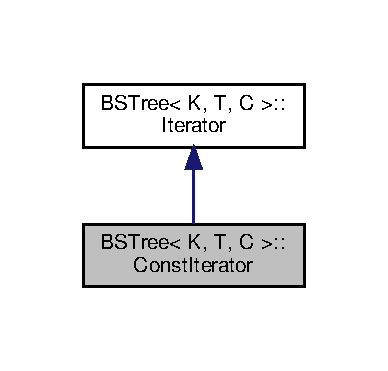
\includegraphics[width=186pt]{class_b_s_tree_1_1_const_iterator__inherit__graph}
\end{center}
\end{figure}


Collaboration diagram for B\+S\+Tree$<$ K, T, C $>$\+:\+:Const\+Iterator\+:\nopagebreak
\begin{figure}[H]
\begin{center}
\leavevmode
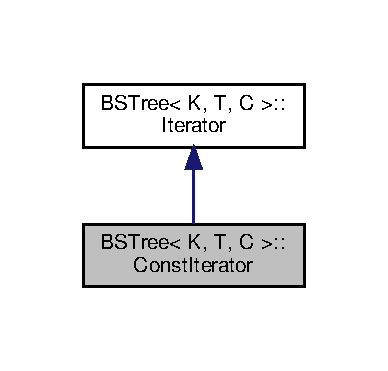
\includegraphics[width=186pt]{class_b_s_tree_1_1_const_iterator__coll__graph}
\end{center}
\end{figure}
\subsection*{Public Types}
\begin{DoxyCompactItemize}
\item 
\mbox{\Hypertarget{class_b_s_tree_1_1_const_iterator_ad1386e8c03ab2942f9b02fce12865b11}\label{class_b_s_tree_1_1_const_iterator_ad1386e8c03ab2942f9b02fce12865b11}} 
using {\bfseries parent} = \hyperlink{class_b_s_tree}{B\+S\+Tree}$<$ K, T, C $>$\+::\hyperlink{class_b_s_tree_1_1_iterator}{Iterator}
\end{DoxyCompactItemize}
\subsection*{Public Member Functions}
\begin{DoxyCompactItemize}
\item 
\mbox{\Hypertarget{class_b_s_tree_1_1_const_iterator_ac402244b14fafd110a847907514d8ecc}\label{class_b_s_tree_1_1_const_iterator_ac402244b14fafd110a847907514d8ecc}} 
const std\+::pair$<$ const K, T $>$ \& {\bfseries operator$\ast$} () const
\end{DoxyCompactItemize}


The documentation for this class was generated from the following file\+:\begin{DoxyCompactItemize}
\item 
/home/w-\/wilson/\+D\+S\+S\+C/first\+\_\+year/exam\+\_\+advanced/test/src/B\+S\+T.\+hpp\end{DoxyCompactItemize}

\hypertarget{structerror}{}\section{error Struct Reference}
\label{structerror}\index{error@{error}}
\subsection*{Public Member Functions}
\begin{DoxyCompactItemize}
\item 
\mbox{\Hypertarget{structerror_a38f200668180ab796773718fda039346}\label{structerror_a38f200668180ab796773718fda039346}} 
{\bfseries error} (const std\+::string \&s) noexcept
\end{DoxyCompactItemize}
\subsection*{Public Attributes}
\begin{DoxyCompactItemize}
\item 
\mbox{\Hypertarget{structerror_acfe267b2efc0e70c21167247824c684c}\label{structerror_acfe267b2efc0e70c21167247824c684c}} 
std\+::string {\bfseries message}
\end{DoxyCompactItemize}


The documentation for this struct was generated from the following file\+:\begin{DoxyCompactItemize}
\item 
/home/w-\/wilson/\+D\+S\+S\+C/first\+\_\+year/exam\+\_\+advanced/test/src/B\+S\+T.\+hpp\end{DoxyCompactItemize}

\hypertarget{class_b_s_tree_1_1_iterator}{}\section{B\+S\+Tree$<$ K, T, C $>$\+:\+:Iterator Class Reference}
\label{class_b_s_tree_1_1_iterator}\index{B\+S\+Tree$<$ K, T, C $>$\+::\+Iterator@{B\+S\+Tree$<$ K, T, C $>$\+::\+Iterator}}


Inheritance diagram for B\+S\+Tree$<$ K, T, C $>$\+:\+:Iterator\+:\nopagebreak
\begin{figure}[H]
\begin{center}
\leavevmode
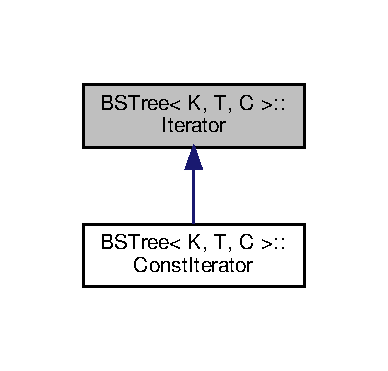
\includegraphics[width=186pt]{class_b_s_tree_1_1_iterator__inherit__graph}
\end{center}
\end{figure}
\subsection*{Public Member Functions}
\begin{DoxyCompactItemize}
\item 
\mbox{\Hypertarget{class_b_s_tree_1_1_iterator_a1b096b8272584f4f4a6671f36b4b2ad3}\label{class_b_s_tree_1_1_iterator_a1b096b8272584f4f4a6671f36b4b2ad3}} 
{\bfseries Iterator} (\hyperlink{class_node_namespace_1_1_b_s_t_node}{B\+S\+T\+Node}$<$ K, T $>$ $\ast$n)
\item 
\mbox{\Hypertarget{class_b_s_tree_1_1_iterator_a359cc7e1b08ebc3754d66c2ba21c9e48}\label{class_b_s_tree_1_1_iterator_a359cc7e1b08ebc3754d66c2ba21c9e48}} 
std\+::pair$<$ const K, T $>$ \& {\bfseries operator$\ast$} () const
\item 
\mbox{\Hypertarget{class_b_s_tree_1_1_iterator_a475c05bcbc2976527931db1376d4207f}\label{class_b_s_tree_1_1_iterator_a475c05bcbc2976527931db1376d4207f}} 
\hyperlink{class_node_namespace_1_1_b_s_t_node}{B\+S\+T\+Node}$<$ K, T $>$ $\ast$ {\bfseries get} ()
\item 
\mbox{\Hypertarget{class_b_s_tree_1_1_iterator_af87e8535c50fc23d7b93ab00e0bba05f}\label{class_b_s_tree_1_1_iterator_af87e8535c50fc23d7b93ab00e0bba05f}} 
\hyperlink{class_b_s_tree_1_1_iterator}{Iterator} \& {\bfseries operator++} () noexcept
\item 
\mbox{\Hypertarget{class_b_s_tree_1_1_iterator_a88df7eda51af41230c5815a7fb137d1b}\label{class_b_s_tree_1_1_iterator_a88df7eda51af41230c5815a7fb137d1b}} 
bool {\bfseries operator==} (const \hyperlink{class_b_s_tree_1_1_iterator}{Iterator} \&other) const noexcept
\item 
\mbox{\Hypertarget{class_b_s_tree_1_1_iterator_ae251c8b6329818c54b3a2094c3501d11}\label{class_b_s_tree_1_1_iterator_ae251c8b6329818c54b3a2094c3501d11}} 
bool {\bfseries operator!=} (const \hyperlink{class_b_s_tree_1_1_iterator}{Iterator} \&other) const noexcept
\end{DoxyCompactItemize}
\subsection*{Private Attributes}
\begin{DoxyCompactItemize}
\item 
\mbox{\Hypertarget{class_b_s_tree_1_1_iterator_aaefde20b1b6b7e8d984c63f909852821}\label{class_b_s_tree_1_1_iterator_aaefde20b1b6b7e8d984c63f909852821}} 
\hyperlink{class_node_namespace_1_1_b_s_t_node}{B\+S\+T\+Node}$<$ K, T $>$ $\ast$ {\bfseries curr\+Node}
\end{DoxyCompactItemize}


The documentation for this class was generated from the following file\+:\begin{DoxyCompactItemize}
\item 
/home/w-\/wilson/\+D\+S\+S\+C/first\+\_\+year/exam\+\_\+advanced/test/src/B\+S\+T.\+hpp\end{DoxyCompactItemize}

\hypertarget{struct_random_key}{}\section{Random\+Key Struct Reference}
\label{struct_random_key}\index{Random\+Key@{Random\+Key}}
\subsection*{Public Member Functions}
\begin{DoxyCompactItemize}
\item 
\mbox{\Hypertarget{struct_random_key_ac3bee095a4fc60b64bcc1e8ea5c2fd45}\label{struct_random_key_ac3bee095a4fc60b64bcc1e8ea5c2fd45}} 
bool {\bfseries operator$<$} (\hyperlink{struct_random_key}{Random\+Key} other) const
\end{DoxyCompactItemize}
\subsection*{Public Attributes}
\begin{DoxyCompactItemize}
\item 
\mbox{\Hypertarget{struct_random_key_a26dbca77342f7c3109d54facfbeb1c2d}\label{struct_random_key_a26dbca77342f7c3109d54facfbeb1c2d}} 
int {\bfseries one}
\item 
\mbox{\Hypertarget{struct_random_key_ad1d15ef83aaf2180176a31222d26f34d}\label{struct_random_key_ad1d15ef83aaf2180176a31222d26f34d}} 
int {\bfseries two}
\item 
\mbox{\Hypertarget{struct_random_key_a727adb496e623fb7e9d4887f16be933f}\label{struct_random_key_a727adb496e623fb7e9d4887f16be933f}} 
int {\bfseries three}
\end{DoxyCompactItemize}


The documentation for this struct was generated from the following file\+:\begin{DoxyCompactItemize}
\item 
/home/w-\/wilson/\+D\+S\+S\+C/first\+\_\+year/exam\+\_\+advanced/test/src/\hyperlink{main_8cc}{main.\+cc}\end{DoxyCompactItemize}

\hypertarget{struct_random_key__explicit}{}\section{Random\+Key\+\_\+explicit Struct Reference}
\label{struct_random_key__explicit}\index{Random\+Key\+\_\+explicit@{Random\+Key\+\_\+explicit}}
\subsection*{Public Attributes}
\begin{DoxyCompactItemize}
\item 
\mbox{\Hypertarget{struct_random_key__explicit_a79914f3641484a20ac0131e37d0d6f2d}\label{struct_random_key__explicit_a79914f3641484a20ac0131e37d0d6f2d}} 
int {\bfseries one}
\item 
\mbox{\Hypertarget{struct_random_key__explicit_a822943d74fc3b07a3c08c340e26c0a8c}\label{struct_random_key__explicit_a822943d74fc3b07a3c08c340e26c0a8c}} 
int {\bfseries two}
\item 
\mbox{\Hypertarget{struct_random_key__explicit_accf813ffe7cbeced0543c1eea0f13f51}\label{struct_random_key__explicit_accf813ffe7cbeced0543c1eea0f13f51}} 
int {\bfseries three}
\end{DoxyCompactItemize}


The documentation for this struct was generated from the following file\+:\begin{DoxyCompactItemize}
\item 
/home/w-\/wilson/\+D\+S\+S\+C/first\+\_\+year/exam\+\_\+advanced/test/src/\hyperlink{main_8cc}{main.\+cc}\end{DoxyCompactItemize}

\chapter{File Documentation}
\hypertarget{_b_s_t_8h}{}\section{/home/w-\/wilson/\+D\+S\+S\+C/first\+\_\+year/exam\+\_\+advanced/test/include/\+B\+ST.h File Reference}
\label{_b_s_t_8h}\index{/home/w-\/wilson/\+D\+S\+S\+C/first\+\_\+year/exam\+\_\+advanced/test/include/\+B\+S\+T.\+h@{/home/w-\/wilson/\+D\+S\+S\+C/first\+\_\+year/exam\+\_\+advanced/test/include/\+B\+S\+T.\+h}}


B\+ST header file.  


{\ttfamily \#include $<$memory$>$}\newline
{\ttfamily \#include $<$utility$>$}\newline
{\ttfamily \#include $<$iostream$>$}\newline
{\ttfamily \#include $<$vector$>$}\newline
{\ttfamily \#include \char`\"{}../src/\+B\+S\+T.\+hpp\char`\"{}}\newline
Include dependency graph for B\+S\+T.\+h\+:\nopagebreak
\begin{figure}[H]
\begin{center}
\leavevmode
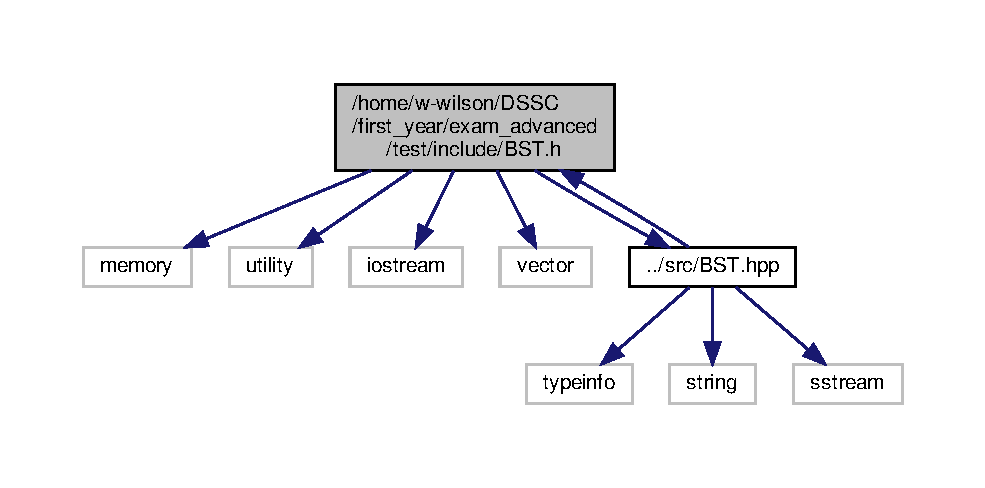
\includegraphics[width=350pt]{_b_s_t_8h__incl}
\end{center}
\end{figure}
This graph shows which files directly or indirectly include this file\+:\nopagebreak
\begin{figure}[H]
\begin{center}
\leavevmode
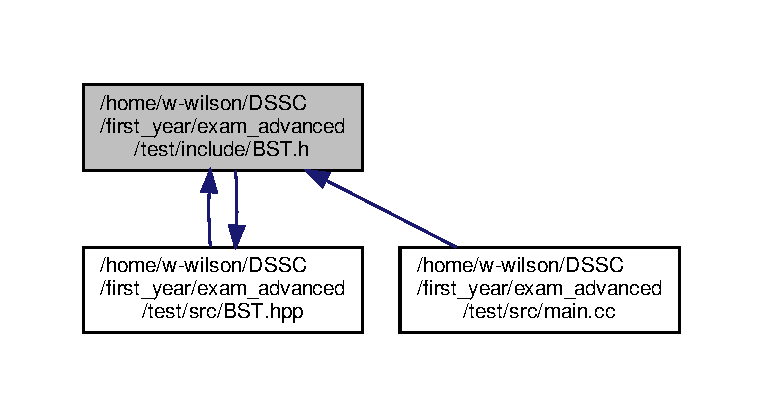
\includegraphics[width=350pt]{_b_s_t_8h__dep__incl}
\end{center}
\end{figure}
\subsection*{Classes}
\begin{DoxyCompactItemize}
\item 
class \hyperlink{class_node_namespace_1_1_b_s_t_node}{Node\+Namespace\+::\+B\+S\+T\+Node$<$ K, T $>$}
\item 
class \hyperlink{class_b_s_tree}{B\+S\+Tree$<$ K, T, C $>$}
\end{DoxyCompactItemize}
\subsection*{Typedefs}
\begin{DoxyCompactItemize}
\item 
\mbox{\Hypertarget{_b_s_t_8h_a2f522589a1f4a4435a4492ebd4f34914}\label{_b_s_t_8h_a2f522589a1f4a4435a4492ebd4f34914}} 
{\footnotesize template$<$typename K , typename T $>$ }\\using {\bfseries B\+S\+T\+Node} = \hyperlink{class_node_namespace_1_1_b_s_t_node}{Node\+Namespace\+::\+B\+S\+T\+Node}$<$ K, T $>$
\end{DoxyCompactItemize}


\subsection{Detailed Description}
B\+ST header file. 

\begin{DoxyAuthor}{Author}
Amadio Simone, Indri Patrick 
\end{DoxyAuthor}
\begin{DoxyDate}{Date}
25/01/19 
\end{DoxyDate}

\hypertarget{main_8cc}{}\section{/home/w-\/wilson/\+D\+S\+S\+C/first\+\_\+year/exam\+\_\+advanced/test/src/main.cc File Reference}
\label{main_8cc}\index{/home/w-\/wilson/\+D\+S\+S\+C/first\+\_\+year/exam\+\_\+advanced/test/src/main.\+cc@{/home/w-\/wilson/\+D\+S\+S\+C/first\+\_\+year/exam\+\_\+advanced/test/src/main.\+cc}}


main file for the exam  


{\ttfamily \#include $<$memory$>$}\newline
{\ttfamily \#include \char`\"{}B\+S\+T.\+h\char`\"{}}\newline
Include dependency graph for main.\+cc\+:\nopagebreak
\begin{figure}[H]
\begin{center}
\leavevmode
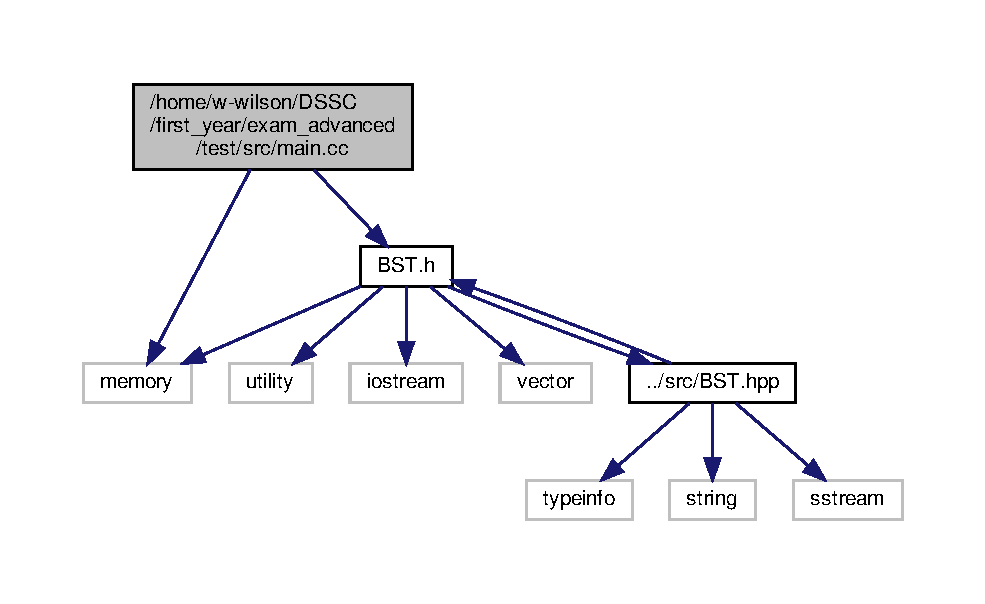
\includegraphics[width=350pt]{main_8cc__incl}
\end{center}
\end{figure}
\subsection*{Classes}
\begin{DoxyCompactItemize}
\item 
struct \hyperlink{struct_random_key__explicit}{Random\+Key\+\_\+explicit}
\item 
struct \hyperlink{structcompareh}{compareh}
\item 
struct \hyperlink{struct_random_key}{Random\+Key}
\end{DoxyCompactItemize}
\subsection*{Functions}
\begin{DoxyCompactItemize}
\item 
\mbox{\Hypertarget{main_8cc_a97d382988fd73ea91bf4c3ffa23c5be8}\label{main_8cc_a97d382988fd73ea91bf4c3ffa23c5be8}} 
std\+::ostream \& {\bfseries operator$<$$<$} (std\+::ostream \&os, const \hyperlink{struct_random_key}{Random\+Key} \&k)
\item 
\mbox{\Hypertarget{main_8cc_ae66f6b31b5ad750f1fe042a706a4e3d4}\label{main_8cc_ae66f6b31b5ad750f1fe042a706a4e3d4}} 
int {\bfseries main} ()
\end{DoxyCompactItemize}


\subsection{Detailed Description}
main file for the exam 

\begin{DoxyAuthor}{Author}
Amadio Simone, Indri Patrick
\end{DoxyAuthor}
\begin{DoxyDate}{Date}
1/2/23 
\end{DoxyDate}

%--- End generated contents ---

% Index
\backmatter
\newpage
\phantomsection
\clearemptydoublepage
\addcontentsline{toc}{chapter}{Index}
\printindex

\end{document}
